\documentclass[11pt]{article}
\usepackage[utf8]{inputenc}
\usepackage[T1]{fontenc}
\usepackage{amsmath,amssymb}
\usepackage{booktabs}
\usepackage{graphicx}
\usepackage{geometry}
\geometry{margin=1in}
\usepackage{authblk}
\usepackage[hidelinks]{hyperref}
\usepackage{caption}

\title{\textbf{Satellite-Derived Drought Indicators as Early Predictors of\\
Food Insecurity Risk in Northern Kenya's Arid and Semi-Arid Lands}}

\author[1]{Craig Carlos Ouma\thanks{%
Correspondence: \texttt{craigcarlos95@gmail.com}. Code and data:
\texttt{github.com/craigouma}}}
\affil[1]{Independent Researcher}
\date{\today}

\begin{document}
\maketitle

\begin{abstract}
\noindent
Food security classifications for Kenya's arid and semi-arid counties are
published roughly three times a year and rest on field assessment. Satellite
rainfall and vegetation data, by contrast, arrive continuously and at no cost to
the user. This paper measures how much of the published classification those
satellite indicators can actually anticipate. Monthly rainfall from CHIRPS
(1981 to 2026) and 16-day vegetation indices from MODIS (2001 to 2026) are
reduced to county means for all 47 Kenyan counties, converted into a
gamma-fitted Standardized Precipitation Index and a Kogan Vegetation Condition
Index, and matched against 2,350 county-period acute food insecurity
classifications published by the Famine Early Warning Systems Network between
2011 and 2026. An XGBoost classifier using only Earth observation features,
evaluated by expanding-window walk-forward validation across 1,363
out-of-sample county-periods, separates Minimal, Stressed, and Crisis-or-worse
classifications with an accuracy of 0.810 (95\,\% interval 0.788 to 0.830) and a
macro-averaged one-versus-rest AUROC of 0.913, against 0.607 for a majority-class
rule. It does not beat persistence, which repeats each county's previous
classification and reaches an accuracy of 0.850. The comparison changes on the
205 county-periods in which the classification actually moved, where persistence
is wrong by construction: the satellite-only model assigns the correct class in
58.5\,\% of them and anticipates the direction of 59.3\,\% of the 113
deteriorations, at a lead of one month, rising to 63.3\,\% at a lead of six
months. Giving the model the previous classification raises its overall accuracy
to 0.824 but cuts deterioration detection to 41.6\,\%, which is a concrete design
warning for any system that blends the two. A SHAP analysis identifies county
identity as the largest single contributor, and among the time-varying
indicators, vegetation condition lagged two months and the six-month rainfall
index. The Vegetation Condition Index value at which the model's contribution to
a Crisis call changes sign, near 18, falls inside the severe vegetation deficit
band that Kenya's National Drought Management Authority already uses
operationally, which is a point of independent agreement between a learned
decision boundary and an established threshold rather than a new one.
\end{abstract}

\section{Introduction}
\label{sec:intro}

Five counties in northern Kenya, Turkana, Marsabit, Samburu, Baringo, and
Wajir, cover 234,733 square kilometres of arid and semi-arid land and receive
between roughly 150 and 450 millimetres of rain a year. Livelihoods there are
predominantly pastoral and depend directly on two short rainy seasons, so a
failed season is not a slow economic drag but a direct loss of pasture, milk,
and herd condition. These counties are where Kenya's drought early warning
system concentrates its attention, and where the Famine Early Warning Systems
Network (FEWS NET) and the National Drought Management Authority publish the
monitoring products that determine when a response is escalated.

Those published classifications arrive on a fixed cycle. FEWS NET has issued
Kenyan acute food insecurity classifications at roughly three reporting dates a
year since 2011, each resting on field assessment, market data, and expert
consensus. Between two reporting dates, a monitoring team has no updated
classification. Satellite rainfall and vegetation data have the opposite
profile: they are updated every month or every 16 days, cover every county
uniformly, cost nothing to obtain, and require no field presence, but they
observe only the physical precursors of food insecurity rather than food
insecurity itself.

This paper asks how far the second can stand in for the first. Specifically, it
asks how much of a published county-level food insecurity classification can be
recovered from satellite rainfall and vegetation data observed before the period
being classified, how much earlier that signal is available, and which
indicators carry it. The question is posed as a forecasting problem throughout:
every predictor is observed at least one month before the period it is used to
classify, and the evaluation never lets a model see a reporting period that
precedes the one it is scored on.

Two design choices shape what follows. First, the model is trained on all 47
Kenyan counties rather than the five study counties alone, because 50 reporting
dates across five counties is too thin a base to fit anything on; the five ASAL
counties remain the subject of the reported results, and are analysed separately
throughout. Second, the model is compared against persistence, meaning a rule
that simply repeats each county's previous published classification. Persistence
is the baseline an operational system actually has to beat, since the previous
bulletin is always in hand, and it is a demanding one: food insecurity phases
are highly autocorrelated. Reporting a satellite model's accuracy without that
comparison would overstate what the model contributes. Section~\ref{sec:results}
reports the comparison in full, including the part where the satellite model
loses.

\section{Background}
\label{sec:background}

\subsection{Vegetation and rainfall indices}

The Vegetation Condition Index of Kogan \cite{kogan1995} rescales the Normalized
Difference Vegetation Index (NDVI) against its own historical range at each
location and time of year:
\begin{equation}
\mathrm{VCI} = 100 \times
\frac{\mathrm{NDVI} - \mathrm{NDVI}_{\min}}
     {\mathrm{NDVI}_{\max} - \mathrm{NDVI}_{\min}},
\label{eq:vci}
\end{equation}
where the minimum and maximum are taken over the historical record for the same
place and the same part of the year. The rescaling is what makes the index
comparable between a dry rangeland and a humid highland: a VCI of 20 means
vegetation is near the low end of what that specific place has shown at that
specific time of year, whatever its absolute greenness. Kenya's National Drought
Management Authority operates on a three-month averaged version of this index,
treating values below 35 as a moderate vegetation deficit sufficient to trigger a
rapid food security assessment, values between 10 and 20 as severe, and values
below 10 as extreme \cite{barrett2020,klisch2016}.

The Standardized Precipitation Index of McKee, Doesken, and Kleist
\cite{mckee1993} performs an analogous rescaling for rainfall. Accumulated
rainfall over a window of one, three, or six months is fitted to a gamma
distribution for each location and calendar month, and the cumulative
probability of an observed total is mapped through the inverse normal
distribution. The result is expressed in standard deviations, negative for
deficit, and is comparable across places with very different rainfall regimes.
The gamma step matters in arid counties, where monthly rainfall is strongly
right-skewed and a plain standardized anomaly misrepresents the dry tail.

\subsection{Prior work on Kenyan drought monitoring}

Klisch and Atzberger \cite{klisch2016} built the operational MODIS NDVI
processing chain that underpins Kenyan drought monitoring, including the
filtering and gap-filling needed to turn 16-day composites into a usable
near-real-time product. Barrett and colleagues \cite{barrett2020} went further
and forecast the three-month VCI itself for Kenyan pastoral counties, reporting
usable skill several weeks ahead, which establishes that the vegetation signal is
partly predictable in its own right.

Ogembo and colleagues \cite{ogembo2026} provide the closest methodological
template to this paper. They combine the Standardized Precipitation
Evapotranspiration Index, VCI, a soil moisture anomaly, and a FAPAR anomaly into
a Combined Drought Indicator for Kenya from 2000 to 2024, classified into
Normal, Watch, Warning, and Alert categories, and report an expansion of the
Alert and Warning classes across the ASALs. Their target is drought severity
itself, constructed from the same physical indicators used as inputs. The
present paper differs in one specific respect that matters for interpretation:
the outcome here is not a drought index but the food insecurity classification
published independently by FEWS NET, which incorporates market, livelihood, and
assessment information that no satellite observes. That makes the prediction
problem harder and the evaluation less circular.

Shukla and colleagues \cite{shukla2021} establish the link this paper depends on
at continental scale, showing that a delayed rainy season onset is a reliable
precursor of low peak NDVI across sub-Saharan Africa, and that the relationship
is strongest in precisely the regions FEWS NET identifies as carrying the
highest acute food insecurity risk. Their result gives a physical reason to
expect rainfall and vegetation anomalies to lead food insecurity outcomes, and
this paper tests how much of that expectation survives contact with the
published classifications county by county.

\section{Data}
\label{sec:data}

Table~\ref{tab:data} summarises the four sources. All are public and none
required an account, a token, or an approval process.

\begin{table}[h]
\centering
\caption{Data sources. Every series was downloaded directly from the cited
public archive; none was simulated, interpolated from a coarser product, or
reconstructed.}
\label{tab:data}
\small
\begin{tabular}{llll}
\toprule
Source & Variable & Resolution & Coverage used \\
\midrule
CHIRPS v2.0 \cite{funk2015} & Monthly rainfall & 0.05 degree & 1981-01 to 2026-08 \\
MOD13Q1 and MYD13Q1 v6.1 & NDVI & 250 m, 16-day & 2001-01 to 2026-08 \\
FEWS NET classifications & IPC-compatible phase & Sub-county units & 2011-01 to 2026-06 \\
HDX Kenya COD-AB & County boundaries & Polygon, 47 counties & 2011 onward \\
\bottomrule
\end{tabular}
\end{table}

\subsection{Rainfall}

CHIRPS combines infrared cold cloud duration estimates with station observations
to produce a gridded rainfall record from 1981 to near-present \cite{funk2015}.
The monthly Africa rasters were clipped to each of the 47 county polygons and
reduced to a county mean, giving 25,756 county-months. The record extends back
to 1981, which allows the climatological baseline to be fixed to the 1981 to
2010 World Meteorological Organization normal period, so that no statistic
computed from the modelling period feeds back into the predictors.

\subsection{Vegetation}

MODIS vegetation indices were read as cloud-optimised GeoTIFFs from the
Microsoft Planetary Computer catalogue, covering the four MODIS sinusoidal tiles
over Kenya. The catalogue serves both the Terra product (MOD13Q1, from 2000) and
the Aqua product (MYD13Q1, from mid-2002); the two are offset by eight days, so
the combined series has an effective eight-day cadence once Aqua is available.
Both were used, and composites were averaged to monthly county means, giving
14,288 county-months.

Two practical points are worth stating. First, each composite was read at a
decimated resolution of roughly 2 km rather than the native 250 m, which keeps
the transfer volume tractable. This choice was checked rather than assumed: over
52 county-composite comparisons, county mean NDVI computed from the decimated
grid differed from the full-resolution value by 0.002 on average, with a maximum
absolute difference of 0.017, which is negligible against county means that range
from 0.15 to 0.68. Second, the MODIS record used here has five missing months
(July to October 2025, and June 2026), which is why one of the 50 FEWS NET
reporting periods drops out of the modelling panel.

The Vegetation Condition Index was computed from equation~\eqref{eq:vci} with the
minimum and maximum taken per county and per calendar month over a 2001 to 2020
baseline, which ends before the fixed test window. Values after 2020 can
therefore fall outside the range 0 to 100 when conditions exceed anything in the
baseline, and they were left unclipped rather than truncated, since truncation
would discard exactly the extreme information the model is meant to use.

\subsection{Outcome variable}

The outcome is the acute food insecurity classification published by FEWS NET
for Kenya, obtained from the FEWS NET Data Warehouse endpoints that the
Humanitarian Data Exchange lists as the public distribution point for this
dataset \cite{fewsnetke}. These are classifications on the Integrated Food
Security Phase Classification scale (1 Minimal, 2 Stressed, 3 Crisis, 4
Emergency, 5 Famine) \cite{ipc2021}, produced for sub-county food security
units on a roughly tri-annual cycle. This is real published classification data,
not a proxy constructed from the predictors used elsewhere in this analysis.

FEWS NET publishes these classifications for livelihood and administrative units
that do not coincide with county boundaries, so an aggregation step is needed.
For each of the 50 reporting dates, the dissolved polygon for each phase was
intersected with each county boundary in an equal-area projection, giving the
share of county area in each phase. The county's label is the phase covering the
largest share of its classified area. Classified area covers 97.1\,\% of county
area on average and never falls below 66.3\,\%, and shares were renormalised onto
the classified part so that unclassified remainder is not silently scored as
Phase 1.

Two properties of this labelling should be kept in view when reading the
results. An area-majority rule understates localised crises: a county where a
quarter of the area is in Crisis and three quarters in Stressed is labelled
Stressed. And the classification is itself an expert product rather than a
measurement, so the model is being asked to predict a considered human judgement,
not a physical quantity.

This gives 2,350 county-periods across 47 counties and 50 reporting dates.
Phase 1 accounts for 1,401, Phase 2 for 749, Phase 3 for 190, and Phase 4 for 10;
no Phase 5 classification appears. Phases 3 and above were merged into a single
Crisis-or-worse class, leaving three classes. Across the five study counties
specifically, 32.7\,\% of county-periods fall in that class, against 8.5\,\%
nationally.

\subsection{Boundaries and licensing}

County boundaries are the Kenya common operational dataset for administrative
boundaries (COD-AB), county level, from the Humanitarian Data Exchange. CHIRPS
is in the public domain, with rights explicitly waived by its producer. NASA
places no restriction on the subsequent use, sale, or redistribution of MODIS
data. FEWS NET distributes the classification data used here under a public data
usage policy, which is recorded in the dataset itself.

\begin{figure}[h]
\centering
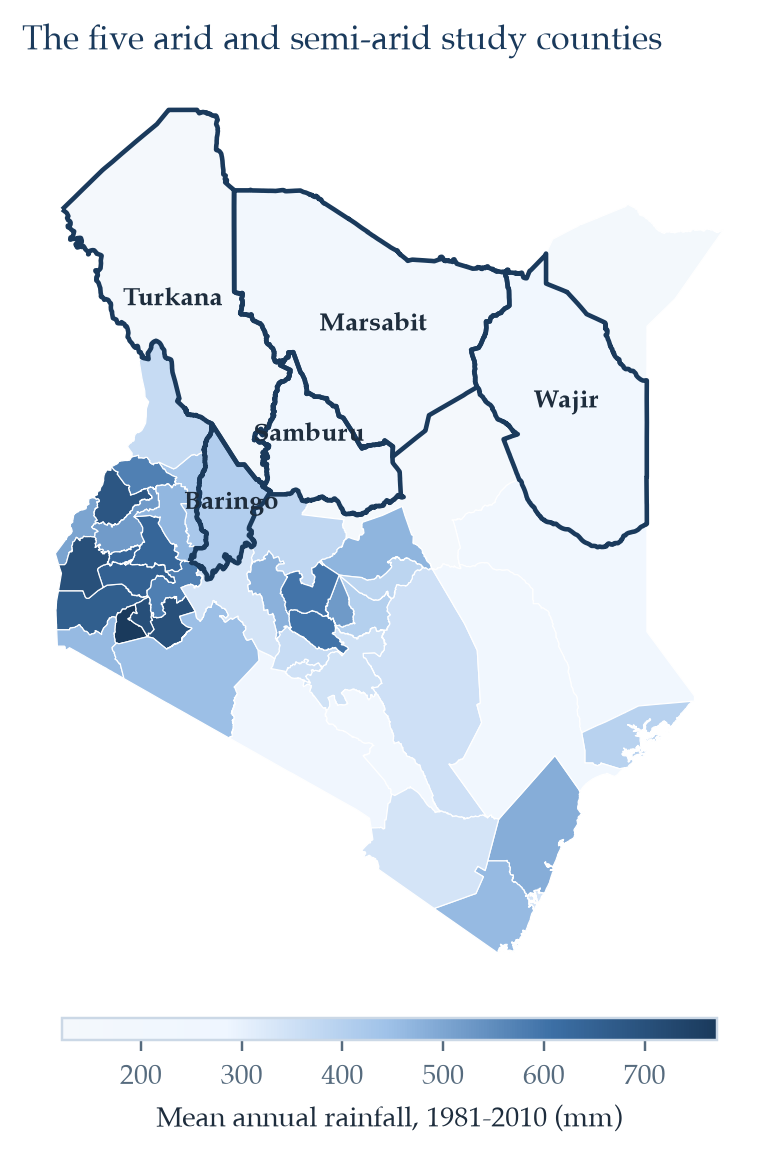
\includegraphics[width=0.72\textwidth]{fig_county_map.png}
\caption{The five study counties within Kenya, shaded by mean annual rainfall
over the 1981 to 2010 baseline. The study counties are among the driest in the
country, and together cover 234,733 square kilometres.}
\label{fig:map}
\end{figure}

\section{Methods}
\label{sec:methods}

\subsection{Features and lead time}

Each row of the modelling panel is one county and one FEWS NET reporting date.
At a lead of $L$ months, the most recent month a feature may draw on is $L$
months before the month the classification describes. The feature set is
deliberately small relative to the number of observations:

\begin{itemize}
\item the one, three, and six month Standardized Precipitation Index at the most
recent usable month, and the three-month index a further two months back;
\item the Vegetation Condition Index at the most recent usable month and at the
two months before it, and the difference between the first and the last of those,
which measures whether vegetation is recovering or still declining;
\item the calendar month and a season indicator distinguishing the long rains
(March to May), the short rains (October to December), and the two dry periods,
since Kenya's rainfall is bimodal;
\item long-run mean annual rainfall for the county, as a measure of structural
aridity, and county identity itself.
\end{itemize}

A lead of one month is the operational case: a monitoring team holding rainfall
and vegetation data through the end of the previous month. Leads of three and
six months answer how much earlier the same signal is usable. At a one-month
lead the panel contains 2,303 county-periods.

\subsection{Model and evaluation}

The classifier is XGBoost \cite{chen2016} with 600 trees of maximum depth four,
a learning rate of 0.05, and subsampling of both rows and columns at 0.8, with
class weights inversely proportional to class frequency. Categorical features
are handled natively. Because the Crisis class is a minority, unweighted
training was also fitted and was worse on every measure reported here, so the
weighted fit is used throughout.

Two evaluation schemes are reported. The first is a single fixed split: train on
reporting periods up to 2020, test on 2021 onward, with the last two training
years held out as an inner validation block for early stopping so that no
test-period information reaches the fitted model. The second, which the paper
treats as primary, is expanding-window walk-forward validation: for each year
from 2016 onward, a model is trained on every reporting period before that year
and predicts that year. This produces 10 folds and 1,363 pooled out-of-sample
predictions covering 2016 to 2026, of which 145 fall in the five study counties.
No model at any point sees a reporting period that comes after the one it is
scored on, and no observation is ever shuffled across time.

\subsection{Baselines}

Three reference points are reported. The majority-class rule predicts Minimal
everywhere. Persistence repeats each county's classification from the previous
reporting date. A third model variant adds that previous classification to the
Earth observation features, which is what an operational system able to use both
would do. A fourth variant drops county identity, to separate the contribution of
the satellite signal from memorised structural vulnerability.

\subsection{Interpretation}

Model behaviour was examined with SHAP \cite{lundberg2017} using the exact tree
explainer. Alongside global importance, the mean SHAP contribution to the
Crisis class was computed within bins of each leading indicator, and the value at
which that contribution changes sign was recorded. That crossing point is the
value at which an indicator starts pushing the model toward a Crisis call rather
than away from it, which makes it the natural candidate for an escalation
trigger.

\section{Results}
\label{sec:results}

\subsection{Overall classification performance}

Table~\ref{tab:main} gives the headline comparison on the pooled walk-forward
predictions. The model using satellite features alone reaches an accuracy of
0.810 with a macro-averaged one-versus-rest AUROC of 0.913, well above the 0.607
that a majority-class rule achieves. Satellite rainfall and vegetation data, observed
before the classification period and with no knowledge of markets, prices,
conflict, or assessment findings, therefore carry a substantial part of the
signal in a published food security classification.

\begin{table}[h]
\centering
\caption{Pooled walk-forward performance, 2016 to 2026, 1,363 out-of-sample
county-periods. Intervals are Wilson score intervals at 95\,\%.}
\label{tab:main}
\small
\begin{tabular}{lcccc}
\toprule
 & Accuracy & Macro F1 & AUROC & Crisis recall \\
\midrule
Majority class          & 0.607 & 0.252 & --    & 0.000 \\
Persistence             & 0.850 & 0.769 & --    & 0.609 \\
EO only, 1 month lead   & 0.810 (0.788, 0.830) & 0.707 & 0.913 & 0.401 \\
EO only, 3 month lead   & 0.809 & 0.717 & 0.911 & 0.417 \\
EO only, 6 month lead   & 0.809 & 0.716 & 0.912 & 0.463 \\
EO plus previous phase, 1 month & 0.824 (0.803, 0.843) & 0.710 & 0.933 & 0.377 \\
EO without county identity, 1 month & 0.775 & 0.664 & 0.896 & 0.358 \\
\bottomrule
\end{tabular}
\end{table}

It also loses to persistence, which reaches 0.850. That result is stated plainly
because it is the honest comparison: a rule that repeats the previous bulletin
outperforms a satellite model that has never been told what the previous
bulletin said. Food insecurity classifications move slowly, and most of the time
the best prediction of the next classification is the last one.

Per-class behaviour, shown in the left panel of Figure~\ref{fig:performance},
is uneven in a way that matters operationally. The model identifies Minimal
county-periods with a precision of 0.95 and a recall of 0.88. For the
Crisis-or-worse class the precision is 0.65 and the recall 0.40, so under a
most-likely-class rule the model misses three fifths of Crisis classifications.
The structure of those misses is more encouraging than the headline number: of
151 Crisis-or-worse county-periods, the model called 60 correctly, 88 Stressed,
and only 3 Minimal. In other words it almost never reads a crisis as normal, and
what it mostly does is understate severity by one step.

\begin{figure}[h]
\centering
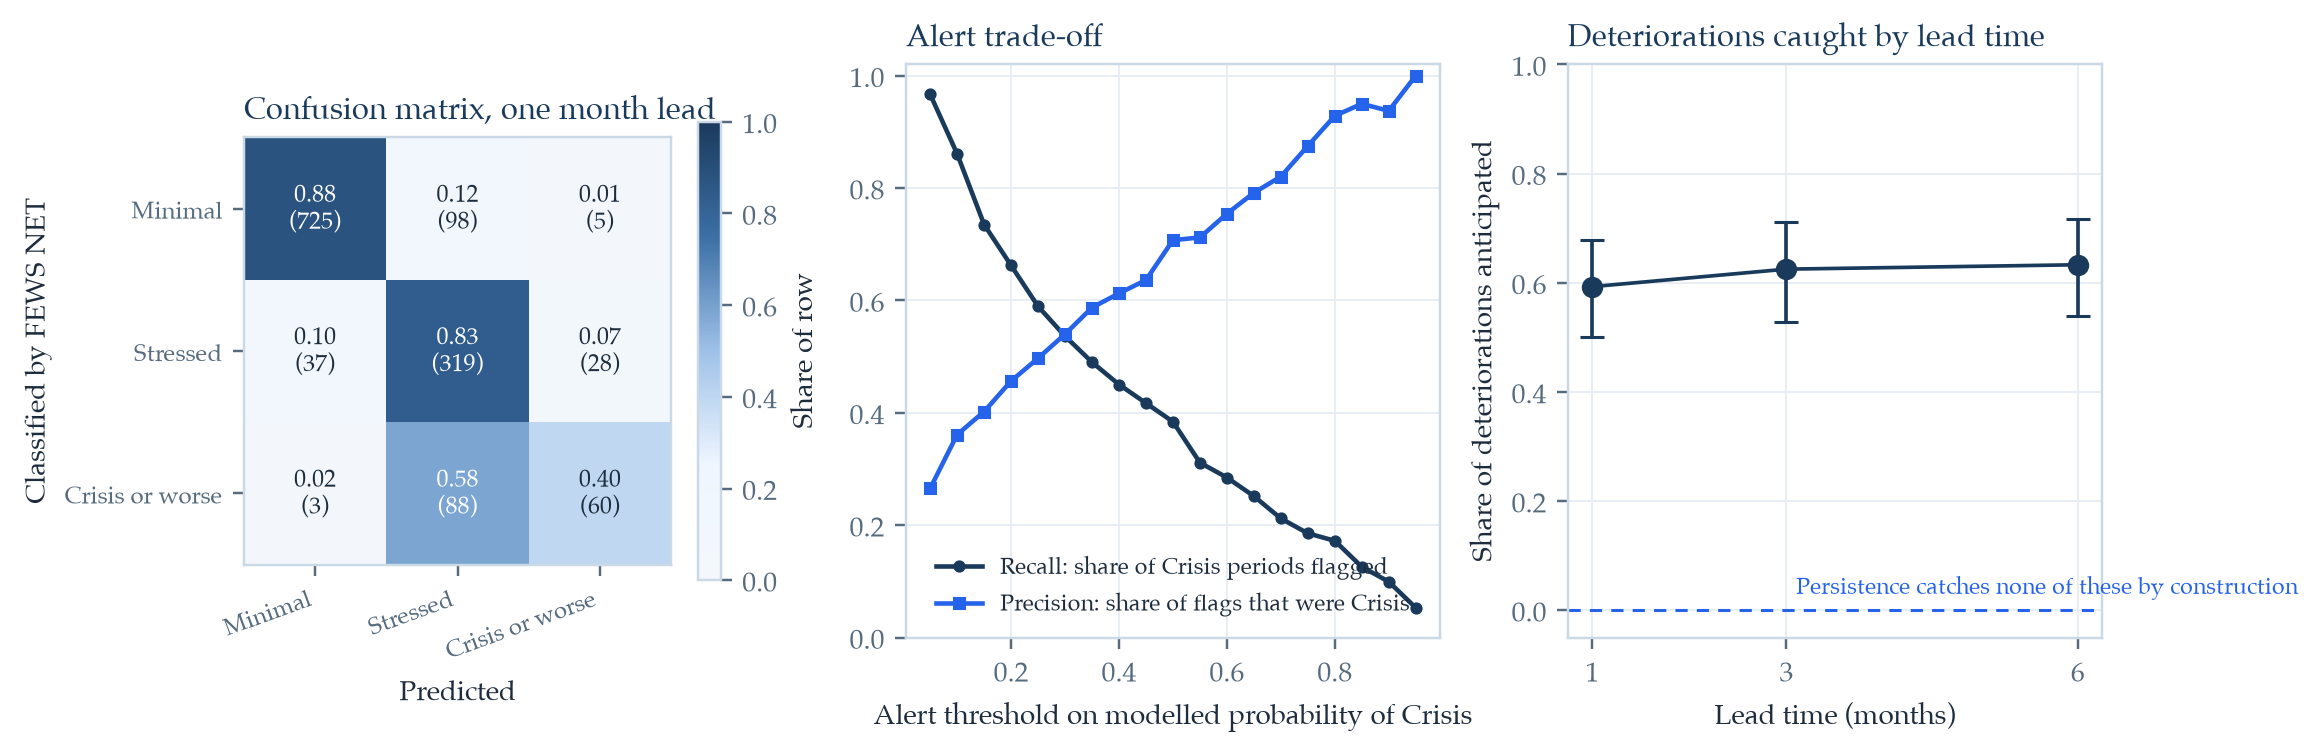
\includegraphics[width=\textwidth]{fig_classification_performance.png}
\caption{Left: confusion matrix at a one-month lead, normalised by row, with
counts in parentheses. Centre: precision and recall for a Crisis alert as the
alert threshold on modelled Crisis probability moves. Right: the share of
deteriorations whose direction the model anticipates, by lead time, with 95\,\%
Wilson intervals; persistence catches none of these by construction.}
\label{fig:performance}
\end{figure}

\subsection{Where the classification changes}

The comparison with persistence inverts once attention moves to the periods
that matter for early warning. Of the 1,363 pooled predictions, the
classification changed from the previous reporting date in 205, and 113 of those
were deteriorations. Persistence is correct on 100\,\% of the stable periods and,
by construction, on none of the 205 changes. The Earth-observation-only model
assigns the correct class in 58.5\,\% of the changes (95\,\% interval 52 to 65),
and anticipates the direction of 59.3\,\% of the deteriorations (50 to 68).

This is the paper's central result. A system built on persistence alone is
accurate in aggregate and silent at exactly the moment a warning would be worth
having. A system built on satellite indicators alone is less accurate in
aggregate and anticipates roughly three fifths of the deteriorations.

\subsection{Lead time}

Performance is close to flat across lead times. Accuracy is 0.810, 0.809, and
0.809 at one, three, and six months, and the share of deteriorations anticipated
is 59.3\,\%, 62.5\,\%, and 63.3\,\% (right panel of Figure~\ref{fig:performance}).
Within the width of the intervals, extending the lead from one month to six
costs nothing.

That is initially counterintuitive and has a straightforward explanation. The
mechanism running from rainfall to food insecurity in a pastoral economy is slow:
a failed rainy season depresses pasture and water availability, herd condition
declines over subsequent months, and the household-level consequences that a food
security assessment records appear later still. A six-month-lagged rainfall index
sits closer to the causal origin of that chain than a one-month-lagged one, and
gains in lead time are not paid for in accuracy. The practical implication is
that the useful warning window here is set by the physical process, not by data
latency.

\subsection{The five study counties}

Restricting the pooled walk-forward predictions to Turkana, Marsabit, Samburu,
Baringo, and Wajir leaves 145 county-periods, of which 65 are Crisis or worse.
Accuracy falls to 0.628, against 0.669 for persistence on the same rows. The
five counties are the hard cases: they carry most of the country's Crisis
classifications, and the three classes are close to balanced there rather than
dominated by Minimal.

Crisis-class precision in these counties is 0.79 with a recall of 0.46, so when
the model calls a Crisis in an ASAL county it is usually right, while still
missing more than half of them under a most-likely-class rule. On the 48 periods
where the classification changed, the model assigns the correct class in
58.3\,\%, and it anticipates the direction of 55.6\,\% of the 27 deteriorations
(95\,\% interval 37 to 72). The interval is wide, and no stronger claim than
"roughly half" is supported by 27 events.

\subsection{Two design choices, tested}

Adding the previous classification to the feature set raises accuracy from 0.810
to 0.824 and AUROC from 0.913 to 0.933. It also cuts the share of deteriorations
anticipated from 59.3\,\% to 41.6\,\% at a one-month lead, and from 63.3\,\% to
35.8\,\% at six months. Given a highly autocorrelated label, the model learns
that copying the previous classification is the cheapest way to reduce loss, and
becomes correspondingly reluctant to call a turning point. An early warning
system that feeds its own previous output back into its model should expect to
buy accuracy at the price of responsiveness.

Dropping county identity costs less than might be expected: accuracy falls from
0.810 to 0.775 and AUROC from 0.913 to 0.896, while deterioration detection
falls only from 59.3\,\% to 54.0\,\%. Most of the model's usable signal is
therefore in the satellite series and the structural rainfall context, not in
memorising which counties are chronically food insecure.

\section{Interpreting the drivers}
\label{sec:drivers}

\subsection{What the model reads}

Figure~\ref{fig:shapbar} and Figure~\ref{fig:beeswarm} show global SHAP
importance and the per-observation distribution of contributions to a Crisis
call. County identity is the largest single contributor by a wide margin (mean
absolute SHAP of 1.16 log-odds against 0.34 for the next feature), which is a
statement about the data rather than about drought: chronic vulnerability is
concentrated, and a model allowed to see county identity will use it. The
sensitivity check in the previous section establishes that it is not doing all
the work.

Among the time-varying indicators the ordering is consistent:

\begin{table}[h]
\centering
\caption{SHAP contribution to the Crisis class, and the indicator value at which
that contribution changes sign, at a one-month lead. Mean absolute SHAP values
are in log-odds.}
\label{tab:shap}
\small
\begin{tabular}{lcc}
\toprule
Indicator & Mean absolute SHAP & Sign change \\
\midrule
County identity                      & 1.162 & -- \\
VCI, two months earlier              & 0.344 & 21.9 \\
SPI-6, most recent month             & 0.261 & $-0.75$ \\
VCI, most recent month               & 0.254 & 18.1 \\
VCI, one month earlier               & 0.244 & 18.2 \\
Mean annual rainfall                 & 0.166 & -- \\
Season                               & 0.141 & -- \\
SPI-1, most recent month             & 0.110 & -- \\
VCI trend over three months          & 0.107 & -- \\
SPI-3, most recent month             & 0.099 & -- \\
\bottomrule
\end{tabular}
\end{table}

Vegetation condition dominates rainfall among the time-varying features, and the
lagged vegetation term carries more weight than the most recent one. This is
consistent with the physical chain described in Section~\ref{sec:results}:
vegetation integrates the rainfall history that matters for pasture, and the
consequences for food security follow the vegetation signal with a delay. Of the
rainfall indices, the six-month accumulation carries roughly two and a half times
the weight of the one-month and three-month versions, which points the same way.
A single poor month tells the model little; two poor seasons tell it a great
deal.

\subsection{Thresholds}

Figure~\ref{fig:dependence} shows the dependence structure for the three leading
time-varying indicators. The VCI relationship is sharply non-linear rather than
gradual. Above roughly 25, the contribution to a Crisis call is flat and
negative. Below roughly 18, it turns positive and rises steeply. The crossing
points for the three VCI terms are 18.1, 18.2, and 21.9, and the six-month
rainfall index crosses at $-0.75$.

These numbers were not chosen; they were read off a model fitted to food
insecurity classifications. It is worth noting where they land. Kenya's National
Drought Management Authority classifies a three-month VCI between 10 and 20 as a
severe vegetation deficit and below 35 as sufficient to trigger a rapid food
security assessment \cite{barrett2020,klisch2016}. The learned boundary near 18
sits inside that severe band. The convergence is independent, since the model was
never shown the NDMA scheme, and it is best read as corroboration of an existing
operational threshold rather than as a new one.

\subsection{From thresholds to alerts}

A most-likely-class rule is not how an early warning system has to be operated.
The centre panel of Figure~\ref{fig:performance} shows the trade-off available by
alerting whenever modelled Crisis probability exceeds a chosen threshold, on the
pooled walk-forward predictions:

\begin{table}[h]
\centering
\caption{Crisis alert trade-off on 1,363 pooled out-of-sample county-periods
containing 151 Crisis-or-worse classifications, one-month lead.}
\label{tab:alert}
\small
\begin{tabular}{lccc}
\toprule
Alert threshold & County-periods flagged & Precision & Recall \\
\midrule
0.10 & 360 & 0.36 & 0.86 \\
0.15 & 276 & 0.40 & 0.74 \\
0.20 & 219 & 0.46 & 0.66 \\
0.30 & 150 & 0.54 & 0.54 \\
0.40 & 111 & 0.61 & 0.45 \\
0.50 &  82 & 0.71 & 0.38 \\
\bottomrule
\end{tabular}
\end{table}

At a threshold of 0.15 the model flags 276 of 1,363 county-periods, about one in
five, and captures 74\,\% of the Crisis-or-worse classifications, with two in five
flags turning out to be correct. Whether that ratio is acceptable depends on what
a flag costs. If it triggers a desk review or a request for a field check, a
60\,\% false alarm rate at one fifth of the country is a reasonable price for
catching three quarters of crises with one to six months of warning. If it
triggers a resource commitment, it is not, and a threshold nearer 0.5 is the
defensible operating point.

Three concrete recommendations follow from the analysis, and each is bounded by
what was actually measured here. First, a VCI below 20 sustained for two
consecutive months is the single most informative satellite trigger available,
and the two-month lag carries more weight than the current month, so a rule
written on sustained deficit rather than instantaneous deficit matches the
model's behaviour. Second, a six-month SPI below $-0.75$ should be treated as a
standing escalation condition, since the six-month accumulation outweighs the
shorter windows by a factor of two and a half. Third, because performance is flat
from one to six months of lead, there is no accuracy argument for waiting; a
county crossing both conditions can be flagged at the earlier point without
penalty.

\begin{figure}[h]
\centering
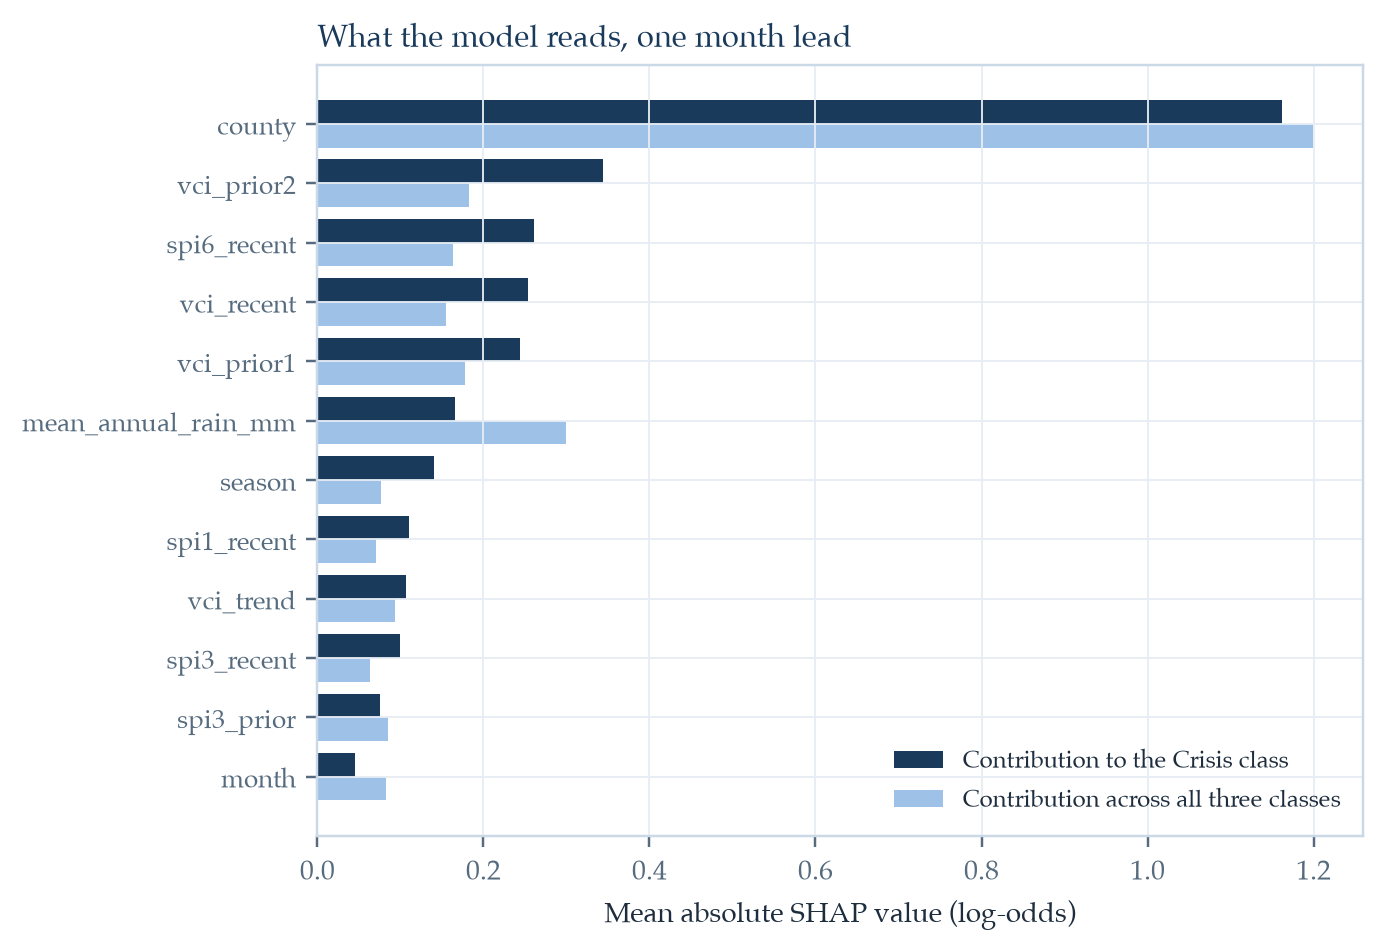
\includegraphics[width=0.78\textwidth]{fig_shap_bar.png}
\caption{Global SHAP importance, one-month lead. Dark bars give the mean
absolute contribution to the Crisis class specifically, light bars the mean
across all three classes.}
\label{fig:shapbar}
\end{figure}

\begin{figure}[h]
\centering
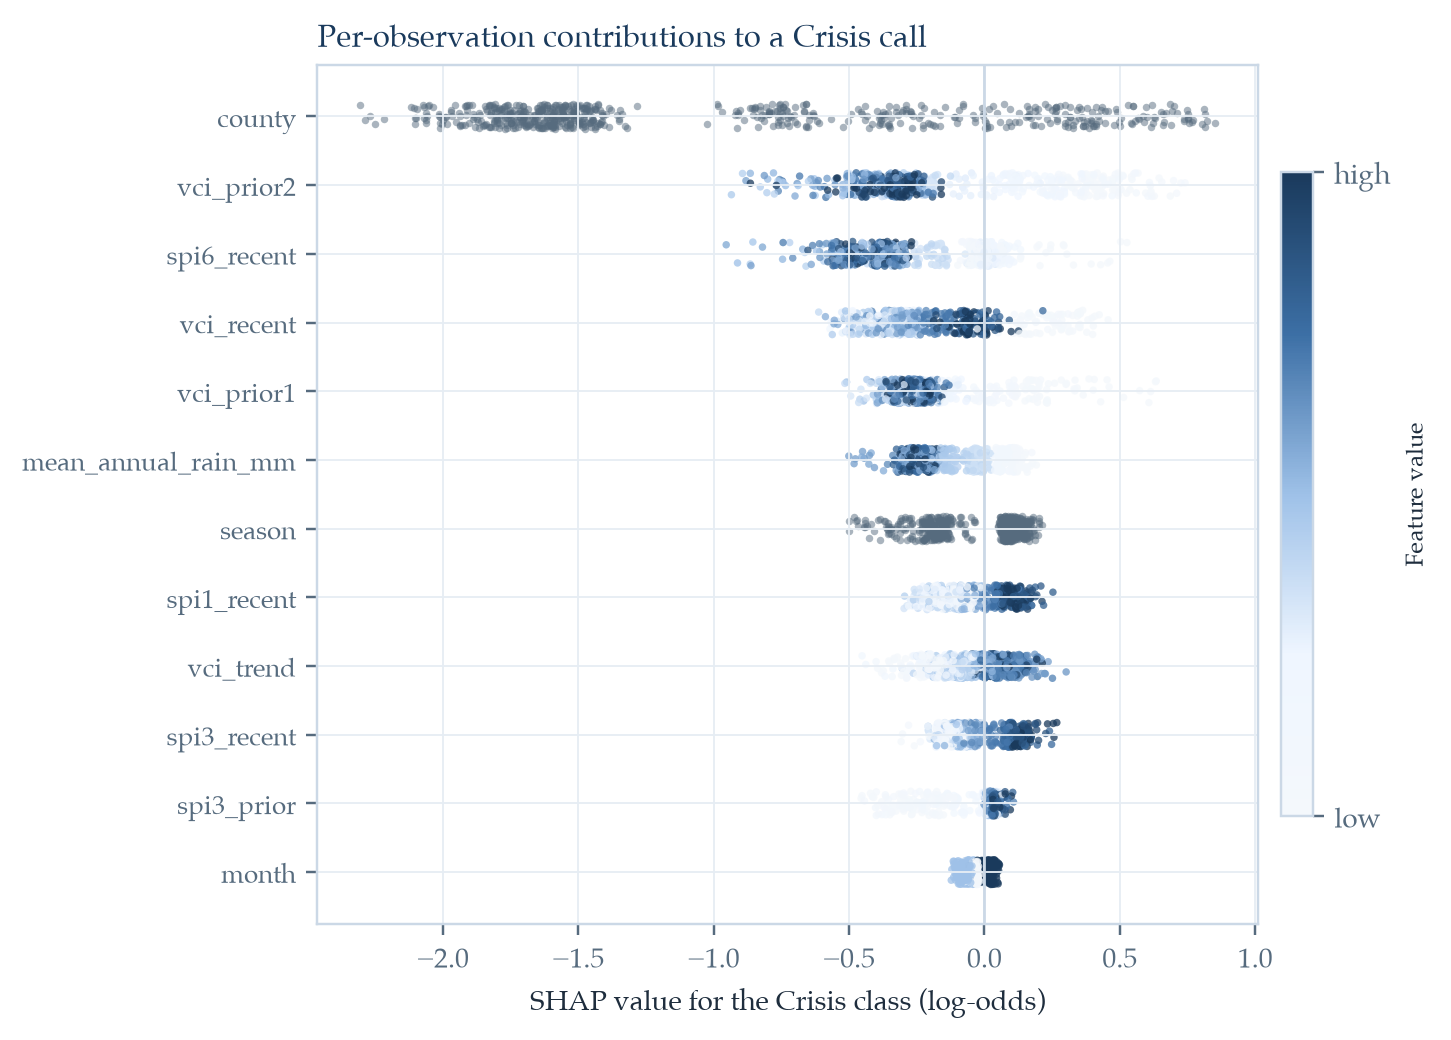
\includegraphics[width=0.85\textwidth]{fig_shap_beeswarm.png}
\caption{Per-observation SHAP contributions to a Crisis call. Points are shaded
by the value of the feature, low to high; categorical features, which have no
low-to-high order, are shown in grey.}
\label{fig:beeswarm}
\end{figure}

\begin{figure}[h]
\centering
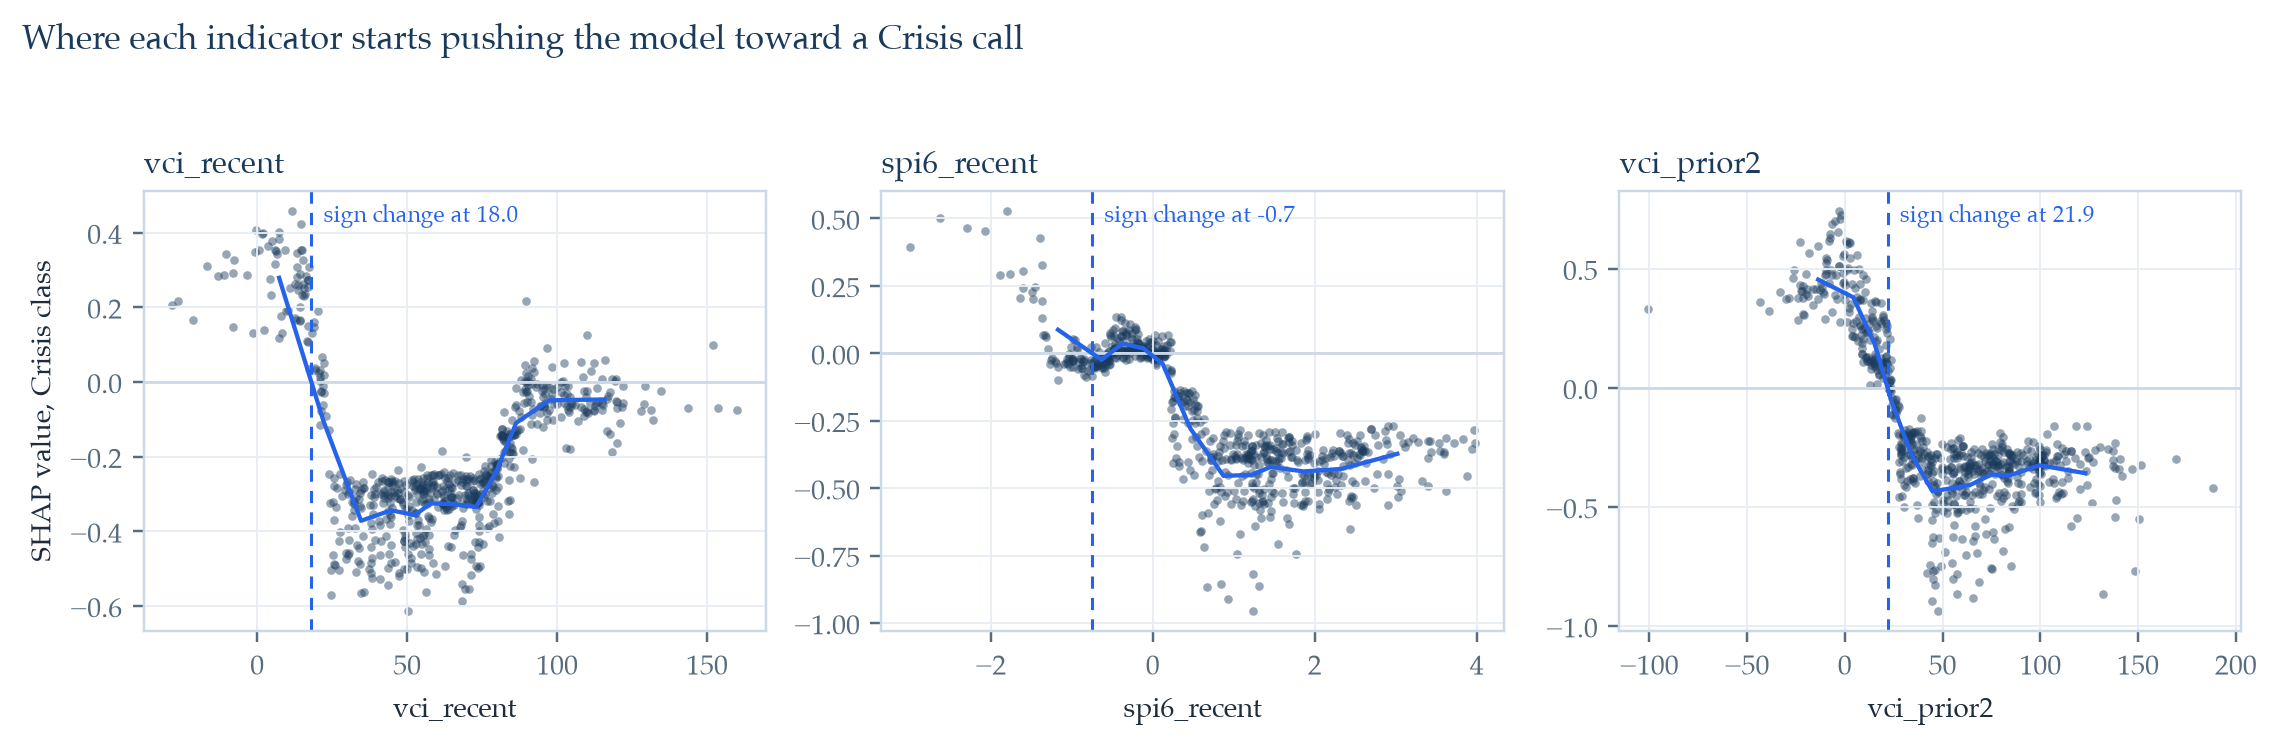
\includegraphics[width=\textwidth]{fig_shap_dependence.png}
\caption{Dependence of the Crisis-class contribution on the three leading
time-varying indicators. The blue line is the binned mean and the dashed line
marks where the contribution changes sign.}
\label{fig:dependence}
\end{figure}

Figure~\ref{fig:timeseries} places these indicators against the classifications
themselves for the five study counties. The 2016 to 2017 and 2021 to 2023 drought
episodes are visible as sustained VCI depressions preceding and accompanying
Crisis classifications, and the 2018 and 2019 to 2020 wet periods as VCI values
at or above the baseline maximum.

\begin{figure}[h]
\centering
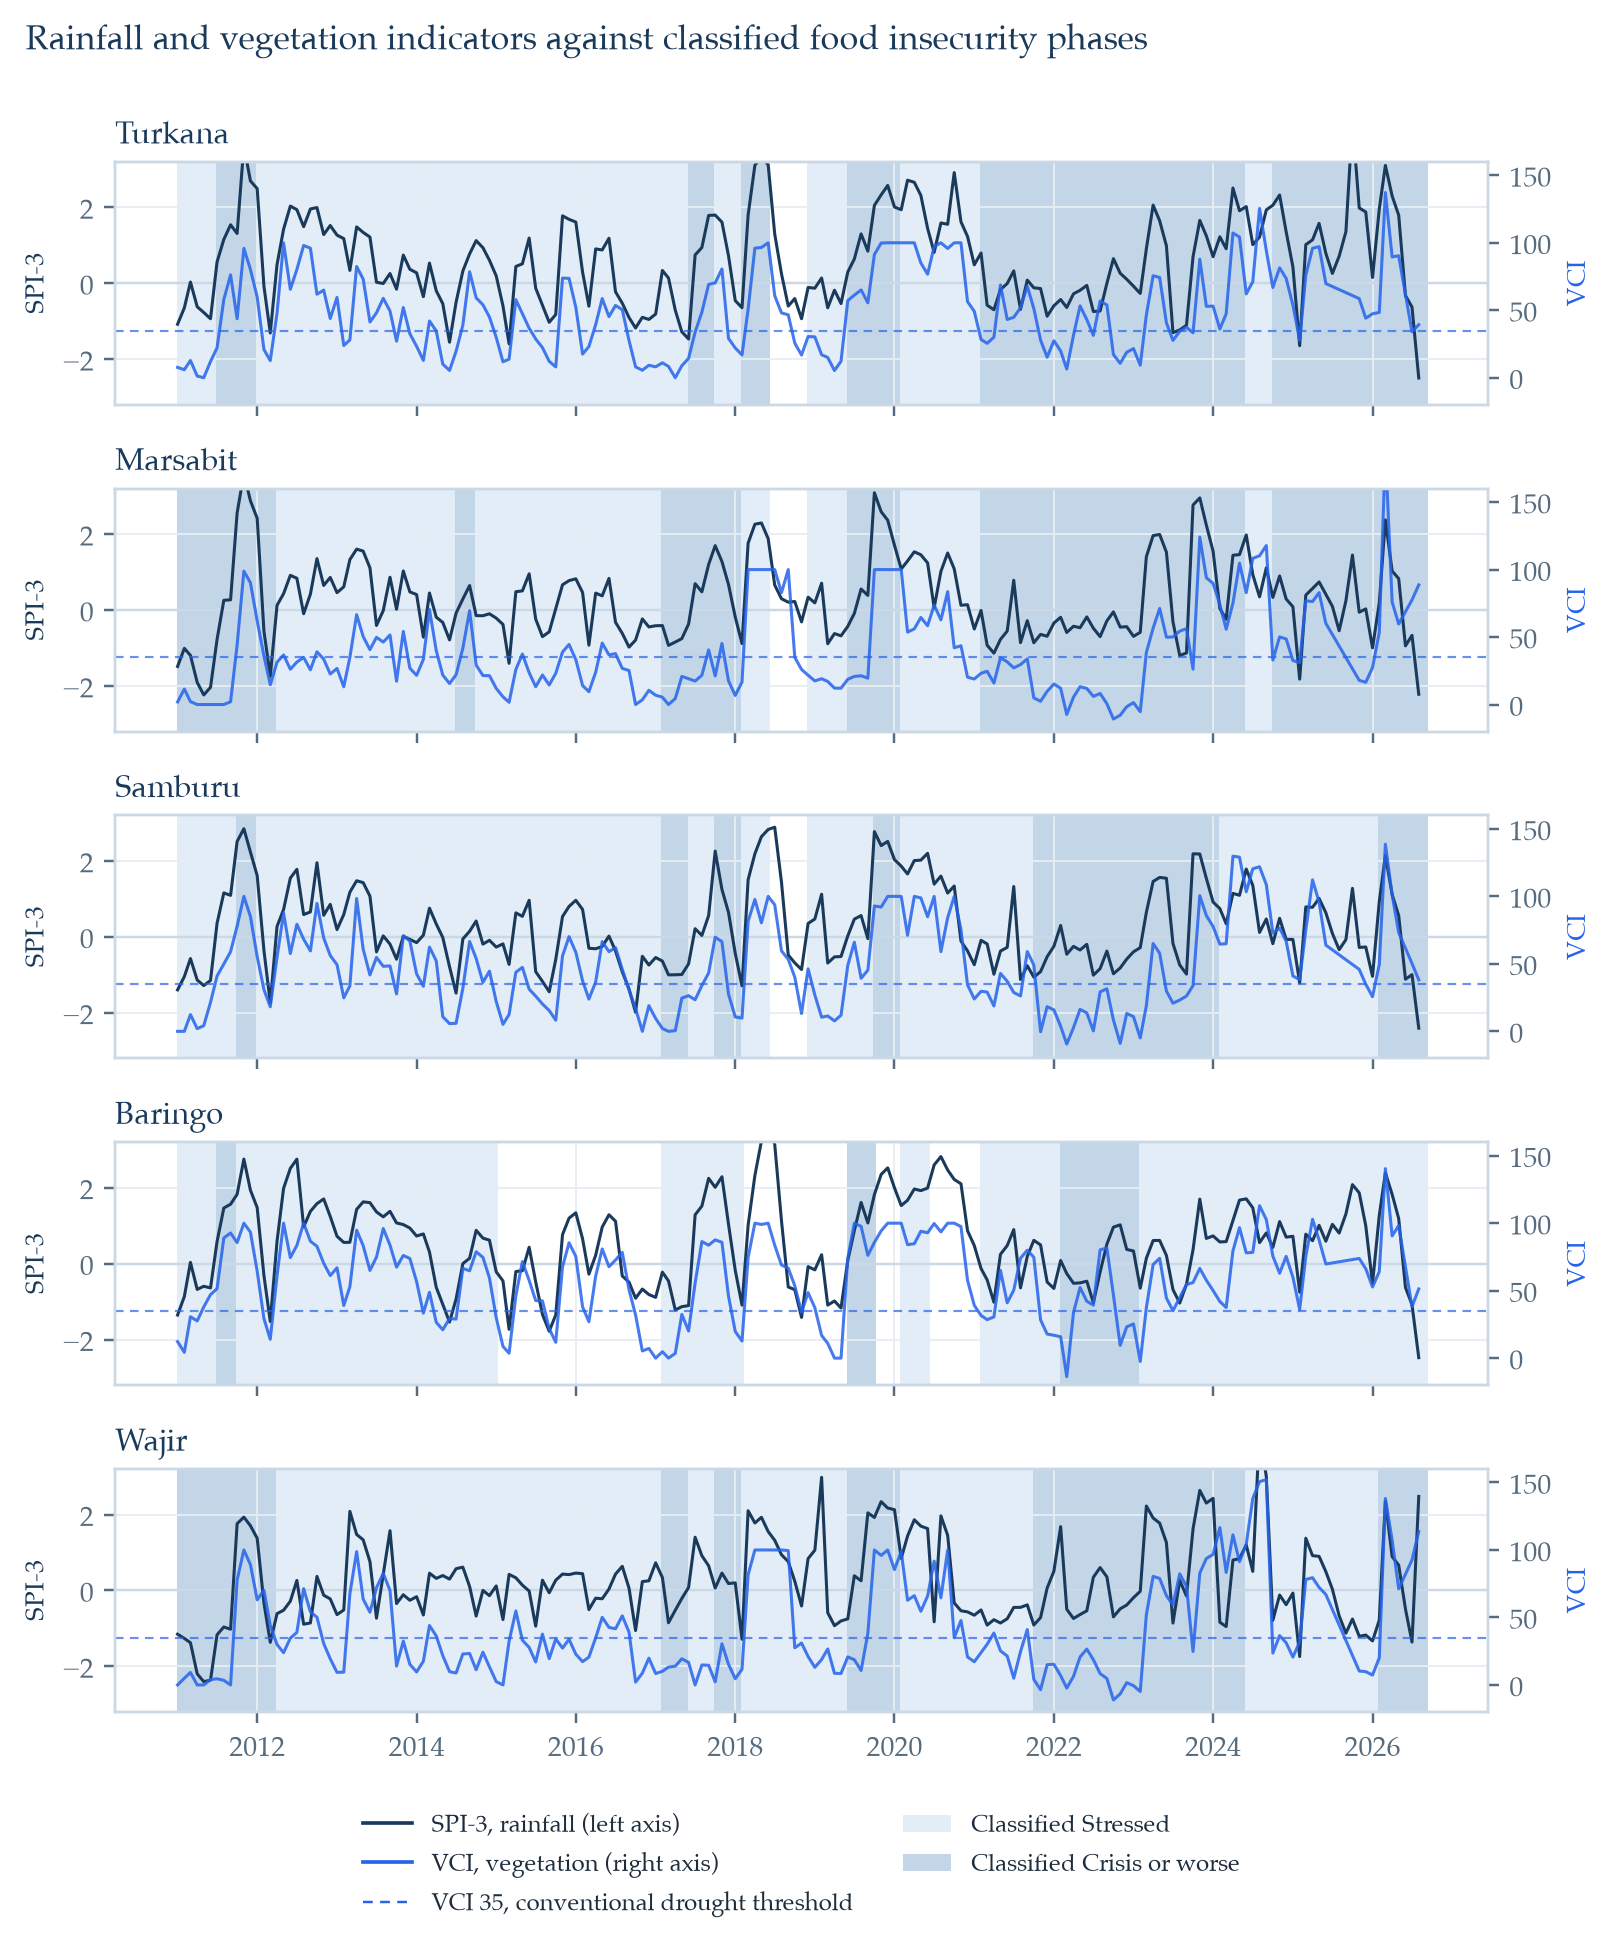
\includegraphics[width=0.92\textwidth]{fig_rainfall_vci_timeseries.png}
\caption{SPI-3 and VCI for the five study counties from 2011, with FEWS NET
classified phases shaded behind them.}
\label{fig:timeseries}
\end{figure}

\section{Limitations}
\label{sec:limitations}

\textbf{The outcome is a judgement, not a measurement.} FEWS NET
classifications are expert products that combine assessment, market, and
livelihood information under a formal protocol. Predicting them is not the same
as predicting food insecurity, and any systematic tendency in how they are
produced is inherited by a model trained on them.

\textbf{The county is a coarse unit.} An area-majority rule assigns one phase to
an entire county, understating localised crises, and FEWS NET's own units are
sub-county for good reason. A county-level model cannot substitute for
household-level assessment and should not be described as identifying
households, communities, or individuals at risk.

\textbf{Satellites do not observe most of the causal chain.} Conflict,
displacement, livestock and staple prices, road access, and the presence or
absence of humanitarian assistance all enter a food insecurity classification and
none is visible in rainfall or vegetation data. The ceiling on a satellite-only
model is set by that omission, and the gap between the model and persistence is
one measure of it.

\textbf{The number of events is small.} The pooled evaluation rests on 151
Crisis-or-worse classifications, 205 phase changes, and 113 deteriorations, and
the study-county figures rest on 27 deteriorations. Intervals are reported
throughout for this reason, and the study-county deterioration rate of 55.6\,\%
has an interval spanning 37 to 72.

\textbf{Two indicator choices are defensible but not unique.} The VCI baseline
runs from 2001 to 2020 and ends before the test window, which avoids leakage but
means post-2020 values can exceed 100. MODIS composites were read at 2 km rather
than 250 m, a choice validated against full resolution to within 0.002 NDVI on
average but not eliminated as a source of difference. Five months of the MODIS
record are missing, removing one of the 50 reporting periods from the panel.

\textbf{The model is trained nationally.} Training on all 47 counties gives the
classifier enough observations to fit, but it means the fitted relationships are
national averages applied to the ASAL counties, where performance is measurably
weaker than it is nationally.

\section{Implications for early warning systems}
\label{sec:implications}

The most useful finding here is not the headline accuracy. It is the division of
labour the comparison exposes. Persistence is an excellent predictor of the next
food security classification and a useless early warning signal, because it never
changes its mind. Satellite indicators are a worse predictor in aggregate and
anticipate around three fifths of deteriorations, one to six months before the
classification changes. These are complementary failure modes, not competing
methods, and the sensible design follows from that: use the published
classification as the state, and use the satellite signal as the trigger for
re-examining it.

The finding that adding the previous classification to the model suppresses
deterioration detection is the operational warning in this paper. A system that
blends its own prior output with new evidence will look better on aggregate
accuracy and will become more conservative at turning points, which is precisely
where the cost of error is highest. If both are used, the satellite trigger
should be evaluated on its own, on the subset of periods where conditions are
changing, rather than on overall accuracy.

The thresholds are the transferable part. A VCI below 20 sustained over two
months and a six-month SPI below $-0.75$ are computable anywhere CHIRPS and MODIS
reach, for any county, at monthly cadence, with no field presence and no data
cost. That these values fall inside bands Kenya's drought authority already uses
suggests the approach is recovering an established operational boundary rather
than inventing one, which is a reason to have more confidence in transferring it
than in replacing what is there.

\section*{Reproducibility statement}

Every number and figure in this paper is produced by the code in the
accompanying repository. The pipeline runs in stages: county boundaries,
CHIRPS rainfall extraction, SPI computation, MODIS NDVI and VCI extraction,
FEWS NET outcome construction, panel assembly, model training and evaluation,
SHAP analysis, and figures. Intermediate county-level series are committed as
CSV files, so the modelling stages can be re-run without repeating the raster
downloads; the raster and MODIS stages re-download from the public archives when
the cached series are absent. Model results are written to
\texttt{model/model\_results.json} and SHAP summaries to
\texttt{model/shap\_summary.json}. Random seeds are fixed. The accompanying
notebook executes the full pipeline end to end. \texttt{DECISIONS.md} records
the substantive choices, including the two departures from the original analysis
plan: Earth observation indicators were extracted for all 47 counties rather than
five, and MODIS was accessed through the Planetary Computer rather than Google
Earth Engine.

\begin{thebibliography}{99}

\bibitem{barrett2020}
Barrett, A. B., Duivenvoorden, S., Salakpi, E. E., Muthoka, J. M., Mwangi, J.,
Oliver, S., and Rowhani, P. (2020). Forecasting vegetation condition for drought
early warning systems in pastoral communities in Kenya. \textit{Remote Sensing
of Environment}, 248, 111886.

\bibitem{chen2016}
Chen, T. and Guestrin, C. (2016). XGBoost: A scalable tree boosting system. In
\textit{Proceedings of the 22nd ACM SIGKDD International Conference on Knowledge
Discovery and Data Mining}, pp. 785-794.

\bibitem{fewsnetke}
Famine Early Warning Systems Network (2026). Kenya current situation acute food
insecurity classifications, 2011 to 2026. FEWS NET Data Warehouse.
\url{https://fews.net/east-africa/kenya}

\bibitem{funk2015}
Funk, C., Peterson, P., Landsfeld, M., Pedreros, D., Verdin, J., Shukla, S.,
Husak, G., Rowland, J., Harrison, L., Hoell, A., and Michaelsen, J. (2015). The
climate hazards infrared precipitation with stations, a new environmental record
for monitoring extremes. \textit{Scientific Data}, 2, 150066.

\bibitem{ipc2021}
IPC Global Partners (2021). \textit{Integrated Food Security Phase
Classification Technical Manual Version 3.1: Evidence and Standards for Better
Food Security and Nutrition Decisions}. Rome.

\bibitem{klisch2016}
Klisch, A. and Atzberger, C. (2016). Operational drought monitoring in Kenya
using MODIS NDVI time series. \textit{Remote Sensing}, 8(4), 267.

\bibitem{kogan1995}
Kogan, F. N. (1995). Application of vegetation index and brightness temperature
for drought detection. \textit{Advances in Space Research}, 15(11), 91-100.

\bibitem{lundberg2017}
Lundberg, S. M. and Lee, S.-I. (2017). A unified approach to interpreting model
predictions. In \textit{Advances in Neural Information Processing Systems 30},
pp. 4765-4774.

\bibitem{mckee1993}
McKee, T. B., Doesken, N. J., and Kleist, J. (1993). The relationship of drought
frequency and duration to time scales. In \textit{Proceedings of the 8th
Conference on Applied Climatology}, American Meteorological Society, Anaheim,
California, pp. 179-184.

\bibitem{ogembo2026}
Ogembo, V., Olala, S., Ronoh, E. K., Mukama, E. B., and Akinyi, G. (2026).
Seasonal drought dynamics in Kenya: remote sensing and combined indices for
climate risk planning. \textit{Climate}, 14(1), 14.

\bibitem{shukla2021}
Shukla, S., Husak, G., Turner, W., Davenport, F., Funk, C., Harrison, L., and
Krell, N. (2021). A slow rainy season onset is a reliable harbinger of drought in
most food insecure regions in Sub-Saharan Africa. \textit{PLOS ONE}, 16(1),
e0242883.

\end{thebibliography}

\end{document}
